\documentclass{memoir}
\usepackage{pgfplots}
\usepgfplotslibrary{external}
\tikzexternalize
\pgfplotsset{width=\textwidth,compat=1.17}
\setSpacing{1.5}

\abnormalparskip{0.2\baselineskip}%
\setlength{\parindent}{1.5cm}%
\renewcommand*{\footnoterule}{\kern -3pt \hrule width 50mm \kern 2.6pt}%

\setstocksize{297mm}{210mm}%
\settrimmedsize{\stockheight}{\stockwidth}{*}
\settrims{0mm}{0mm}
\setlrmarginsandblock{30mm}{20mm}{*}%
\setulmarginsandblock{30mm}{20mm}{*}%
\setheadfoot{\baselineskip}{2\baselineskip}
\setheaderspaces{20.0mm}{*}{*}%
\setmarginnotes{2.0mm}{16mm}{5.0mm}%
\setcolsepandrule{3.5mm}{0.15mm}
\setfootins{\bigskipamount}{\bigskipamount}
\checkandfixthelayout[fixed]
\begin{document}
\chapter{}
\begin{figure}[ht]
  \pgfplotsset{width=0.5\textwidth,compat=1.17}
  \centering%
  \begin{tikzpicture}[baseline,trim axis left]%
     \begin{axis}[%
          title={Graph made from numerical FORTRAN data.}, %
          xlabel={$x$}, %
          ylabel={$y$}, %
          scatter, %
          %only mark,%
          mark size = 0.6pt, %
          enlargelimits=true,%
          %colorbar,%
          legend style = {%
                    cells = {anchor = east},%
                    legend pos = north west%
                    },%
          ]%
          \addplot [domain = -10:10,samples = 25] table {outputplot.dat};
     \end{axis}%
  \end{tikzpicture}%
  %\caption{Gr\'afico para uma fun\c{c}\~ao quadr\'atica a partir a solução num\'erica obtida com FORTRAN. Número de pontos plotados: 25.}\label{fig:A.a.1}%
  %
  \hskip 10pt%
  %
  %\centering%
  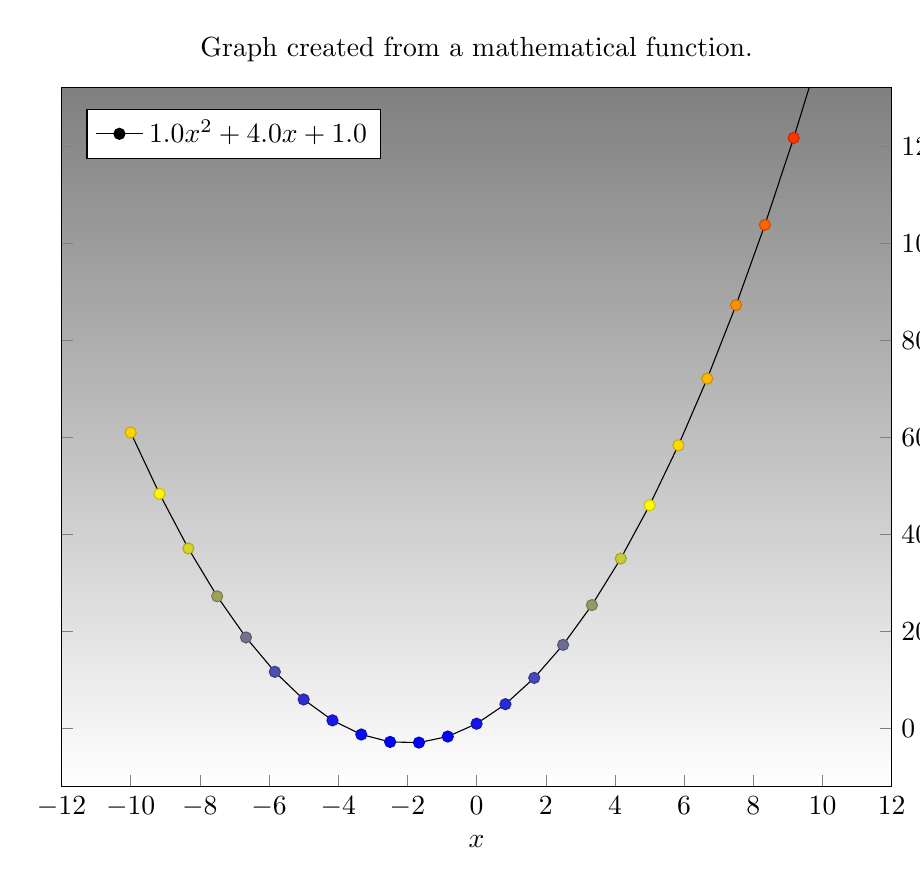
\begin{tikzpicture}[baseline,trim axis right]%
    \begin{axis}[%
          title={Graph created from a mathematical function.}, %
          xlabel={$x$},%
          scatter, %
          %only mark,%
          %mark size=1.0pt, %
          enlargelimits=true, %
          colorbar, %
          axis background/.style = {%
                    shade, %
                    top color =  gray, %
                    bottom color = white%
                    }, %
          legend style = {%
                    cells = {anchor = east},%
                    legend pos = north west%
                    },%
          %domain = -10:10,%
          %image = 0:120,%
          xmin = -10,%
          xmax =  10,%
          %minor x tick num = 2,%
          ymin = 0,%
          ymax = 120,%
          %minor y tick num = 1,%
          yticklabel pos = upper,%
          ]%
      \addplot[%
          domain  = -10:10,%
          samples = 25,%
      ]{1.0*x^2 + 4.0*x + 1.0};%
      \addlegendentry{$1.0x^2 + 4.0x + 1.0$}%
    \end{axis}%
  \end{tikzpicture}%
  %\caption{Plotado a partir da expressão}\label{fig:A.a.2}
\end{figure}
\end{document} 